%++++++++++++++++++++++++++++++++++++++++
\documentclass[letterpaper,12pt]{article}
\usepackage{tabularx} % extra features for tabular environment
\usepackage{amsmath}  % improve math presentation
\usepackage{graphicx} % takes care of graphic including machinery
\usepackage[margin=1in,letterpaper]{geometry} % decreases margins
\usepackage{cite} % takes care of citations
\usepackage[final]{hyperref} % adds hyper links inside the generated pdf file
\usepackage[T1]{fontenc} %polish letters
\usepackage{caption} %captions
\usepackage{fancyvrb} % no idea what it is
\usepackage[polish]{babel} % polish date
\usepackage{listings} % R code
\usepackage{float} % jakjaś pozycja obrazka H
\usepackage{hyperref} % links

\hypersetup{
	colorlinks=true,       % false: boxed links; true: colored links
	linkcolor=blue,        % color of internal links
	citecolor=blue,        % color of links to bibliography
	filecolor=magenta,     % color of file links
	urlcolor=blue
}
%++++++++++++++++++++++++++++++++++++++++


\begin{document}
% figure caption pattern
\captionsetup[figure]{labelfont={bf},labelformat={default},labelsep=period,name={Rys.}}
% table caption pattern
%\captionsetup[table]{labelfont={bf},labelformat={default},labelsep=period,name={Tab.}}
\pagestyle{plain}

% tytuł
\title{Porównanie rzeczywistego zasięgu pokrywy lodowej na obszarze Antarktydy z modelem matematycznym}
\author{Maciej Bąk, Hubert Długosz, Filip Giermek}
\date{\today}
\maketitle

% wstęp
\section{Wstęp}
Realizowanym zadaniem było wykonanie wykresów obrazujących rzeczywisty zasięg pokrywy lodowej na obszarze Antarktydy w latach 1978 - 2009, oraz stworzenie modelu matematycznego będącego reprezentacją zasięgu rzeczywistego, a następnie porównanie uzyskanych wyników.

\section{Charakterystyka danych}
Do stworzenia projektu posłużono się danymi zebranymi w formie tabeli przedstawiającymi za pomocą współrzędnych geograficznych zasięg pokrywy lodowej w kolejnych dniach w~ww.~okresie.

\section{Wykonanie}
Całość projektu została wykonana w środowisku programistycznym R. Najistotniejsze narzędzia z których skorzystano w celu przetworzenia oraz wizualizacji danych:

\begin{itemize}
  \item biblioteka plotly (wizualizacja współrzędnych biegunowych)
  \item biblioteka orca (zapisanie wykresów)
  \item pakiet FFmpeg (stworzenie animacji)
\end{itemize}

\section{Minimalny zasięg lodu w analizowanym okresie}

W celu odtworzenia rzeczywistego kształtu Antarktydy znaleziono dla każdego kąta długości geograficznej w badanym okresie najmniejszą wartość zasięgu pokrywy lodowej. Znalezione, a następnie przetworzone dane, posłużyły do stworzenia wykresu obrazującego kształt kontynentu. \newline Biorąc pod uwagę fakt, że dane przedstawione są w formie współrzędnych geograficznych, w celu uzyskania wykresu przedstawiającego rzeczywisty kształt Antarktydy z perspektywy bieguna południowego, należało je odpowiednio przekształcić tj.:
\begin{itemize}
  \item uzyskać wartość bezwzględną kątów - wszystkie wartości były ujemne, wynika to z~położenia obszaru na półkuli południowej.
  \item odjąć wartości od kąta 90 stopni - dzięki temu środek wykresu przesunął się z równika na biegun.
\end{itemize}

Efekt powyższych działań przedstawia Rysunek 1.

\begin{figure}[ht]
        \centering 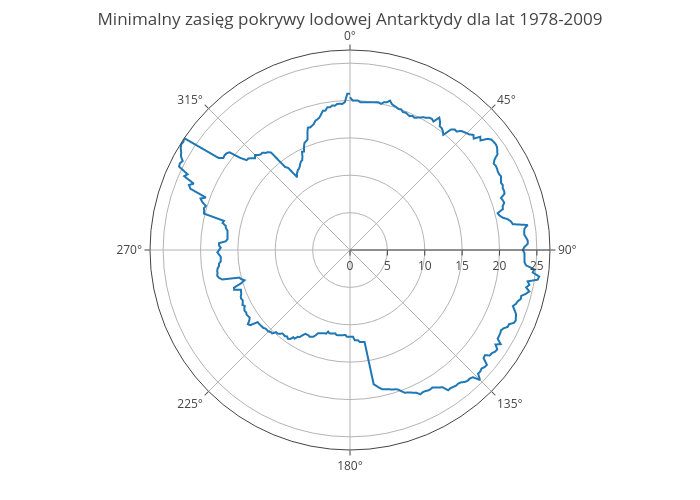
\includegraphics[width=1\columnwidth]{minimalIceRange.png}
        \caption{
                \label{fig:samplesetup}
                Kontur minimalnego zasięgu lodu
        }
\end{figure}

\section{Uproszczony model zasięgu lodu w czasie}
% napisać jakieś coś ala wstęp%
% 360 osobnych modeli
Pracę rozpoczęto od wyświetlenia punktów odpowiadających jednemu stopniowi długości geograficznej na wykresie. Analizując rozkład punktów, zdecydowano o zastosowaniu regresji liniowej z wykorzystaniem funkcji okresowych, jakimi są sinus i cosinus. Zmienną zależną jest zasięg lodu, a zmienną niezależną wartości sinusa i cosinusa. Ostateczne dopasowanie danych wykonano poprzez odpowiednie zastosowanie funkcji \textit{lm()} jako \textit{lm(angle~xc+xs)}.



\newpage
\begin{figure}[ht]
        \centering \includegraphics[width=1\columnwidth]{wyk_punktowy.jpg}
        \caption{
                \label{fig:samplesetup}
                Wykres punktowy przed dopasowaniem modelu
        }
\end{figure}


\noindent W czasie przeprowadzania analizy zauważono różnicę w interwałach czasowych między wartościami. Po uwzględnieniu tego aspektu, wykonano ostateczne dopasowanie funkcji tym samym tworząc model zasięgu lodu w funkcji czasu.
\newline

\begin{figure}[H]
        \centering \includegraphics[width=1\columnwidth]{wyk_lin.png}
        \caption{
                \label{fig:samplesetup}
                Uproszczony model dla jednej z wartości długości geograficznej
        }
\end{figure}

\noindent Oś pozioma wykresów przedstawia zmienną TimeSeq będącą reprezentacją kolejnych dni poddawanych analizie. Wykonano 360 analogicznych modeli, biorąc pod uwagę każdy kąt długości geograficznej. Uzyskane modele użyto do wizualizacji wymodelowanego zasięgu arktycznego lodu.

%%%%%%%%%%%%%%%%%%%%%%%%%%%%%%%%%%%%%%%%%%%%%%%%%%%%%%%%%%%%%%%%
\section{Rozszerzony model zasięgu lodu w czasie}

Podjęto próbę stworzenia modelu który lepiej dopasuje się do danych rzeczywistych. Kompleksowe rozwiązanie problemu powstało poprzez zastosowanie regresji wielomianowej. Wykorzystano wielomian dwóch zmiennych stopnia 25. Ponownie zastosowano funkcję \textit{lm()}, tym razem w postaci \textit{lm(z $\sim$ poly(x, y, degree = 25), data = df)}. Rys. 4. przedstawia dane rzeczywiste, Rys. 5. przedstawia dane wymodelowane przy wykorzystaniu powyższej funkcji dla całego okresu badań.


%rzeczywisty
\begin{figure}[ht]
        \centering 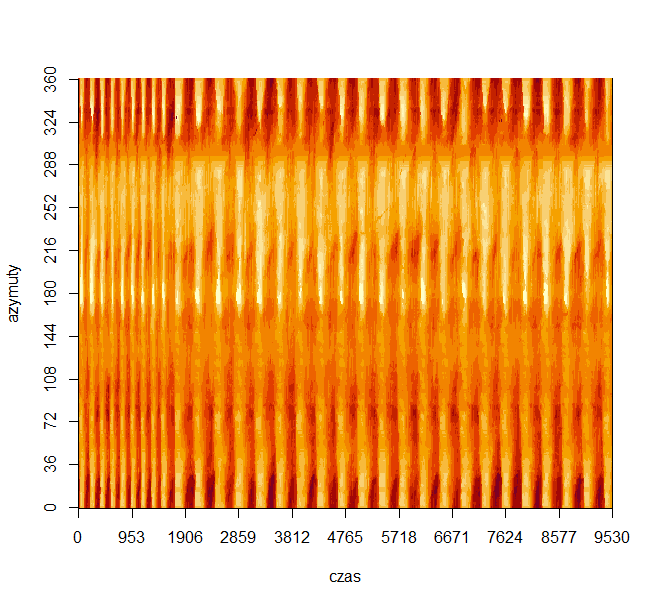
\includegraphics[width=0.7\columnwidth]{plotData.png}
        \caption{
                \label{fig:samplesetup}
                Wizualizacja danych rzeczywistych
        }
\end{figure}

\newpage

%model
\begin{figure}[h]
        \centering 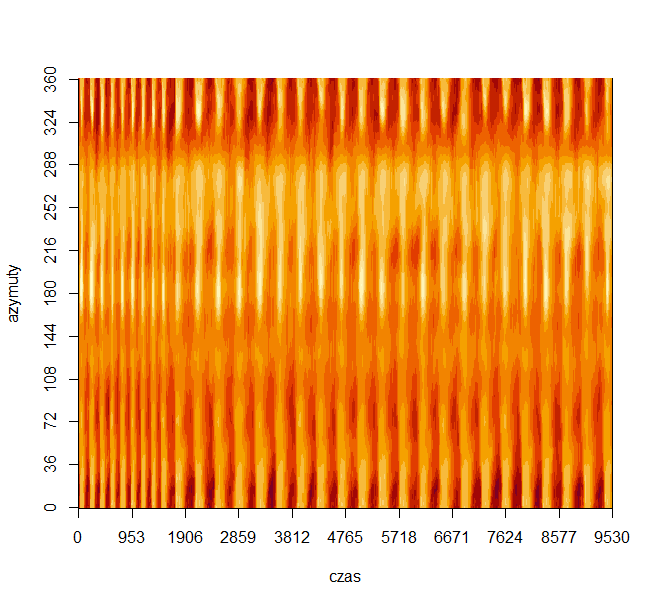
\includegraphics[width=0.7\columnwidth]{plotModel.png}
        \caption{
                \label{fig:samplesetup}
                Model odpowiadający danym z Rys. 4
        }
\end{figure}

%model
\begin{figure}[h!]
        \centering \includegraphics[width=0.7\columnwidth]{plotRazemRok.png}
        \caption{
                \label{fig:samplesetup}
                Porównanie obrazu danych rzeczywistych do modelu dla jednego roku pomiarów
        }
\end{figure}




\newpage
\section{Wizualizacja modelu}

Przygotowano funkcję \textit{plotDoubleIce}, która tworzyła wykres obrazujący rzeczywisty i wymodelowany zasięg lodu dla danej daty. Kolejno, łączyła ze sobą dwa wykresy i dodawała tytuł będący reprezentacją daty dla danego modelu. Kluczowym było zwrócenie uwagi na fakt, że wykresy narysowane bezpośrednio z danych nie były prawidłowo zorientowane - konieczne okazało się odpowiednie ich odwrócenie, tak aby zgadzały się z przyjęta konwencją obrazowania obszarów okołobiegunowych. Obrazy numerowano zachowując kolejność dat. W~ten sposób powstało 9530 obrazów ,które wymagały połączenia. W tym celu wykorzystano pakiet \texit{FFmpeg} będący otwartoźródłowym projektem umożliwiającym edytowanie multimediów. Funkcję \texit{ffmpeg}, z odpowiednio dobranymi argumentami wywołano w terminalu. Jako rezultat powstały filmy obrazujące zmienność rzeczywistego i wymodelowanego zasięgu pokrywy lodowej w czasie.

\begin{figure}[ht]
        \centering \includegraphics[width=0.75\columnwidth]{model2.png}
        \caption{
                \label{fig:samplesetup}
                Przykładowy rzeczywisty i wymodelowany zasięg
        }
\end{figure}


\section{Podsumowanie}

% Model będący rezultatem wykonywanego zadania w głównej mierze pokrywa się z zasięgiem rzeczywistym. Występują jednak względnie spore niedoskonałości, które widać przy szybkiej zmianie powierzchni rzeczywistej. Wynika to z przyjętego modelu który jest sporym uproszczeniem realnej sytuacji. Zachowuje jednak zmienność powierzchni lodu w czasie. Kod źródłowy i dokumentacja projektu wraz z filmem będącym rezultatem pracy zamieszczony został w repozytorium \href{https://github.com/kerness/Antarctica-Ice-Range}{Antarctica-Ice-Range\footnote{https://github.com/kerness/Antarctica-Ice-Range}}.



Model uproszczony w głównej mierze pokrywa się z zasięgiem rzeczywistym. Występują jednak względnie spore niedoskonałości, które widać przy szybkiej zmianie powierzchni rzeczywistej. Wynika to z przyjętego modelu, który jest sporym uproszczeniem realnej sytuacji. Zachowuje jednak zmienność powierzchni lodu w czasie. Zdecydowanie lepszy rezultat dało podejście z wykorzystaniem modelu rozszerzonego, gdzie zasięg rzeczywisty i wymodelowany w zdecydowanie większym stopniu pokrywają się. Różnica dopasowania wartości dobrze widoczna jest poprzez porównanie stworzonych animacji. Kod źródłowy i dokumentacja projektu wraz z animacjami będącymi rezultatami pracy zamieszczone zostały w repozytorium \href{https://github.com/kerness/Antarctica-Ice-Range}{Antarctica-Ice-Range\footnote{https://github.com/kerness/Antarctica-Ice-Range}}.

%++++++++++++++++++++++++++++++++++++++++
% References section will be created automatically
% with inclusion of "thebibliography" environment
% as it shown below. See text starting with line
% \begin{thebibliography}{99}
% Note: with this approach it is YOUR responsibility to put them in order
% of appearance.


\renewcommand\refname{Bibliografia}
\begin{thebibliography}{99}


\bibitem{stack}
Sine curve fit using lm and nls in R,
\\\texttt{stackoverflow.com/questions/20104680/sine-curve-fit-using-lm-and-nls-in-r}

\bibitem{plotly}
Plotly R Open Source Graphing Library,
\\\texttt{plotly.com/r/}

\bibitem{ffmpeg}
FFmpeg Documentation,
\\\texttt{ffmpeg.org/ffmpeg.html}

\bibitem{ffmpeg}
Fitting polynomial regression,
\\\texttt{https://datascienceplus.com/fitting-polynomial-regression-r/}

\bibitem{ffmpeg}
Polynomial Regression in R Programming,
\\\texttt{https://www.geeksforgeeks.org/polynomial-regression-in-r-programming/}



\end{thebibliography}







\end{document}
